% !TEX root = poster.tex
% Symposium poster -- UChicago DSI Summer Lab 2026.
% Build:  ./build.sh          (latexmk + biber; see README.md)
% Every number carries a comment naming the repo file it came from; see README.md.
\documentclass[14pt, margin=1in, innermargin=15mm,
               blockverticalspace=8mm, colspace=16mm,
               subcolspace=10mm]{tikzposter}

% 36in x 24in landscape. `portrait` cancels the width/height swap the class's
% `landscape` option hands to geometry; the explicit sizes are final.
\geometry{portrait, paperwidth=36in, paperheight=24in, margin=1in}

% tikzposter freezes its usable text box at class-load time, i.e. at A0. Redo
% that one calculation now that the paper is 36in x 24in, or every block is laid
% out for a sheet the poster is not printed on. This is why `innermargin` above
% is a normal positive length rather than the large negative value tikzposter
% templates often use to stretch the frozen A0 width out to their real sheet.
\makeatletter
\setlength{\TP@visibletextwidth}{\textwidth-2\TP@innermargin}
\setlength{\TP@visibletextheight}{\textheight-2\TP@innermargin}
\makeatother

\usepackage[utf8]{inputenc}
\usepackage{amsmath}
\usepackage{amssymb}
\usepackage{graphicx}
\usepackage{adjustbox}
\usepackage{enumitem}
\usepackage{microtype}

\usepackage{uwtheme}

\usepackage{biblatex}
\addbibresource{ref.bib}

% set theme parameters
\tikzposterlatexaffectionproofoff
\usetheme{UWTheme}
\usecolorstyle{UWStyle}

\usepackage[scaled]{helvet}
\renewcommand\familydefault{\sfdefault}
\usepackage[T1]{fontenc}

\definecolor{tbdcolor}{HTML}{B25900}

% A numbered sub-question badge. The same badge marks the question and its
% answer, so the two-part structure is findable without reading any body text.
% Two variants because the theme's block titles are white-on-red bars: \badge
% for white backgrounds, \badgeontitle for the red title bar.
\newcommand{\badge}[1]{%
  \tikz[baseline=(b.base)]{
    \node[circle, fill=UWDarkRed, text=white, inner sep=5mm, font=\bfseries]
      (b) {#1};}}
\newcommand{\badgeontitle}[1]{%
  \tikz[baseline=(b.base)]{
    \node[circle, fill=white, text=UWRed, inner sep=5mm, font=\bfseries]
      (b) {#1};}}

% A pending result. Sized and positioned as the finished content will be, so
% the layout does not move when the number lands.
\newcommand{\tbdblock}[3]{%
  \begin{tikzpicture}
    \node[draw=tbdcolor, line width=2pt, dash pattern=on 10pt off 8pt,
          rounded corners=5pt, inner sep=7mm, align=left, anchor=north west,
          text width=\dimexpr\linewidth-18mm\relax, minimum height=#1] at (0,0)
      {{\color{tbdcolor}\bfseries TBD\ \ }\textbf{#2}\\[4mm]#3};
  \end{tikzpicture}}

\title{Is there signal in the vascular networks?}
\author{Spencer Venancio\ \ \textbullet\ \ Advisor: Dr.\ Anna Woodard}
\institute{University of Wisconsin--Madison}

\makeatletter
\newcommand\insertlogoi[2][]{\def\@insertlogoi{\includegraphics[#1]{#2}}}
\newcommand\insertlogoii[2][]{\def\@insertlogoii{\includegraphics[#1]{#2}}}
\newlength\LogoSep
\setlength\LogoSep{0pt}

\insertlogoi[height=1.35in]{uw_madison_logo.pdf}
\insertlogoii[height=1.0in]{dsi_logo.png}

\renewcommand\TP@maketitle{%
   \centering
   \begin{minipage}[b]{0.62\linewidth}
        \centering
        \color{titlefgcolor}
        {\bfseries \Huge \sc \@title \par}
        \vspace*{0.35em}
        {\huge \@author \par}
        \vspace*{0.35em}
        {\LARGE \@institute}
    \end{minipage}%
    \tikz[remember picture,overlay]\node[anchor=south east,xshift=0.5\linewidth,inner sep=0pt] {%
       \@titlegraphic
    };
}

\renewcommand\maketitle[1][]{  % #1 keys
    \normalsize
    \setkeys{title}{#1}
    % Title dummy to get title height
    \node[transparent,inner sep=\TP@titleinnersep, line width=\TP@titlelinewidth, anchor=north, minimum width=\TP@visibletextwidth-2\TP@titleinnersep]
        (TP@title) at ($(0, 0.5\textheight-\TP@titletotopverticalspace)$) {\parbox{\TP@titlewidth-2\TP@titleinnersep}{\TP@maketitle}};
    \draw let \p1 = ($(TP@title.north)-(TP@title.south)$) in node {
        \setlength{\TP@titleheight}{\y1}
        \setlength{\titleheight}{\y1}
        \global\TP@titleheight=\TP@titleheight
        \global\titleheight=\titleheight
    };

    % Compute title position
    \setlength{\titleposleft}{-0.5\titlewidth}
    \setlength{\titleposright}{\titleposleft+\titlewidth}
    \setlength{\titlepostop}{0.5\textheight-\TP@titletotopverticalspace}
    \setlength{\titleposbottom}{\titlepostop-\titleheight}

    % Title style (background)
    \TP@titlestyle

    % Title node
    \node[inner sep=\TP@titleinnersep, line width=\TP@titlelinewidth, anchor=north, minimum width=\TP@visibletextwidth-2\TP@titleinnersep]
        at (0,0.5\textheight-\TP@titletotopverticalspace)
        (title)
        {\parbox{\TP@titlewidth-2\TP@titleinnersep}{\TP@maketitle}};

    \node[inner sep=0pt,anchor=west]
      at ([xshift=-\LogoSep]title.west)
      {\@insertlogoi};

    \node[inner sep=0pt,anchor=east]
      at ([xshift=\LogoSep]title.east)
      {\@insertlogoii};

    % Settings for blocks
    \normalsize
    \setlength{\TP@blocktop}{\titleposbottom-\TP@titletoblockverticalspace}
}
\makeatother

% begin document
\begin{document}
\maketitle

%% ------------------------------------------------- motivation + question ---
\block{Why vessels, and what we asked}{
  \begin{minipage}[t]{0.46\linewidth}
    Breast tumours are treated with chemotherapy \emph{before} surgery. Patients
    who reach \textbf{pCR} --- pathologic complete response, no residual invasive
    cancer at surgery --- do markedly better, and knowing early who will get
    there would let clinicians change course while it still matters.

    \vspace{3mm}
    Tumours recruit their own blood supply, and \textbf{DCE-MRI} --- dynamic
    contrast-enhanced MRI --- images the breast repeatedly while a contrast agent
    washes through it. We ask whether the vessel network, not the tumour, carries
    the response signal.
  \end{minipage}\hfill
  \begin{minipage}[t]{0.50\linewidth}
    {\fontsize{32}{38}\selectfont\bfseries\color{UWDarkRed}
      Is there signal in the vascular networks?}

    \vspace{3mm}
    \badge{1}\ \ {\fontsize{25}{31}\selectfont\bfseries Is there signal in the
      blood vessels at all?}

    \vspace{3mm}
    \badge{2}\ \ {\fontsize{25}{31}\selectfont\bfseries Does the graph add
      anything beyond that?}

    \vspace{3mm}
    The two answers stay separate. Collapsing them into one ``our model works''
    claim would hide which half is doing the work.
  \end{minipage}
}

%% ------------------------------------------- methods and the two answers ---
\begin{columns}
\column{0.30}
\block{From scan to prediction}{
  \begin{tikzfigure}[Ultrafast DCE-MRI to vessel graph to prediction, on one real
    case. Panels 1--4 are measured data; panel 5 is schematic.]
    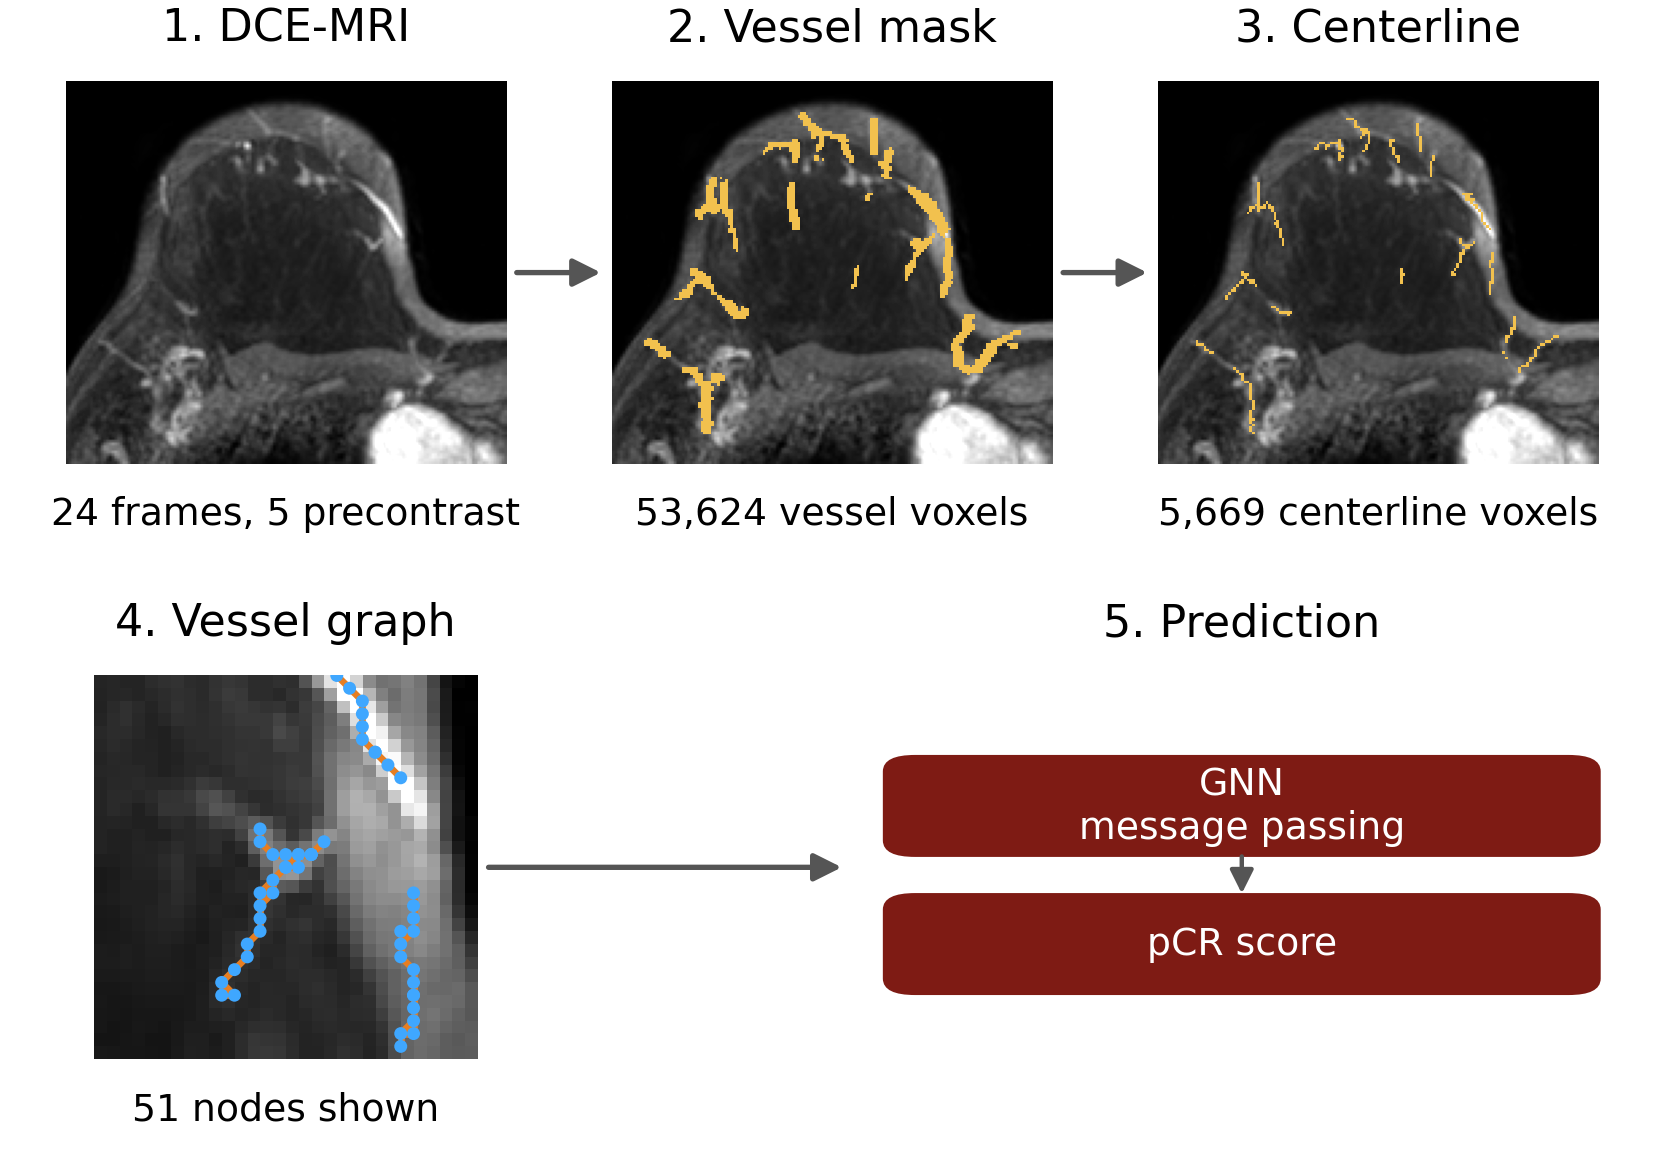
\includegraphics[width=\linewidth]{pipeline.png}
  \end{tikzfigure}

  \vspace{2mm}
  One real case: 24 frames over 119.5\,s, 5 of them before contrast arrives.
  % experiments/dce_curve_example/README.md
  A \textbf{centerline} is the one-voxel-wide skeleton down the middle of each
  segmented vessel; every centerline voxel becomes a graph node. Segmentation and
  centerline extraction are upstream lab pipeline.
}

\block{What the graph is}{
  \textbf{Nodes.} Three representations, built from the same skeleton and compared
  on identical folds: one node per \emph{centerline voxel}, per \emph{vessel
  segment}, or at \emph{branch points and tips}.

  \vspace{2mm}
  \begin{center}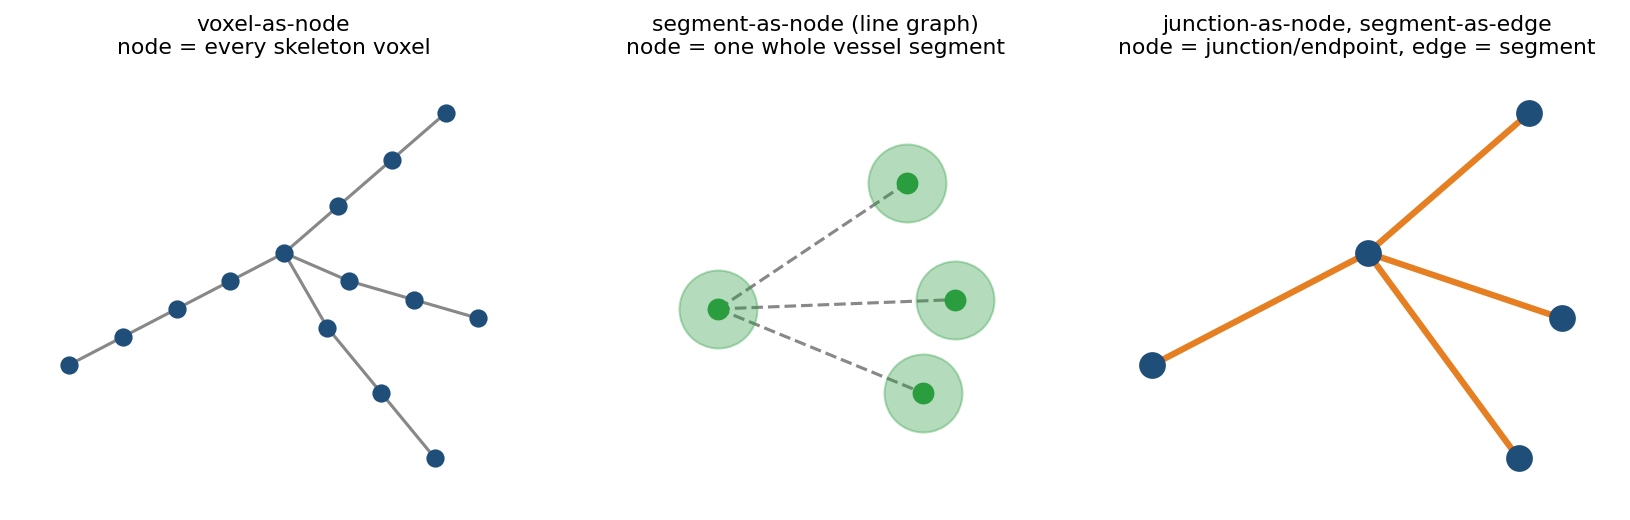
\includegraphics[width=0.74\linewidth]{graph_representations.png}\end{center}

  \vspace{2mm}
  \textbf{Edges.} Voxel adjacency, a shared branch point, or the segments
  themselves, kept as a multigraph.

  \vspace{3mm}
  \textbf{Node features (7).} Peak time \textbullet\ peak enhancement
  \textbullet\ time to enhancement \textbullet\ wash-in slope \textbullet\
  wash-out slope \textbullet\ positive AUC \textbullet\ vessel radius.
  \textbf{Edge features} summarise each segment's geometry and mean kinetics.

  \vspace{3mm}
  \textbf{What is thrown away.} Each node's 24-point enhancement curve becomes
  six scalars before the model sees it, and edges carry no flow direction --- so
  the graph can only average static per-node kinetics.
}

\column{0.40}
\block{Contrast-forecasting pretraining}{
  {\color{UWRed}\bfseries A new contribution of this project.}

  \vspace{3mm}
  The models here never see contrast \emph{move}. So we pretrain the encoder on a
  label-free task: \textbf{given the first frames, predict every node's
  enhancement over the next frames}, using message passing --- so the encoder has
  to learn how the bolus propagates along vessels. After
  \textcite{tang2022ssl}, who forecast EEG.

  \vspace{2mm}
  \begin{center}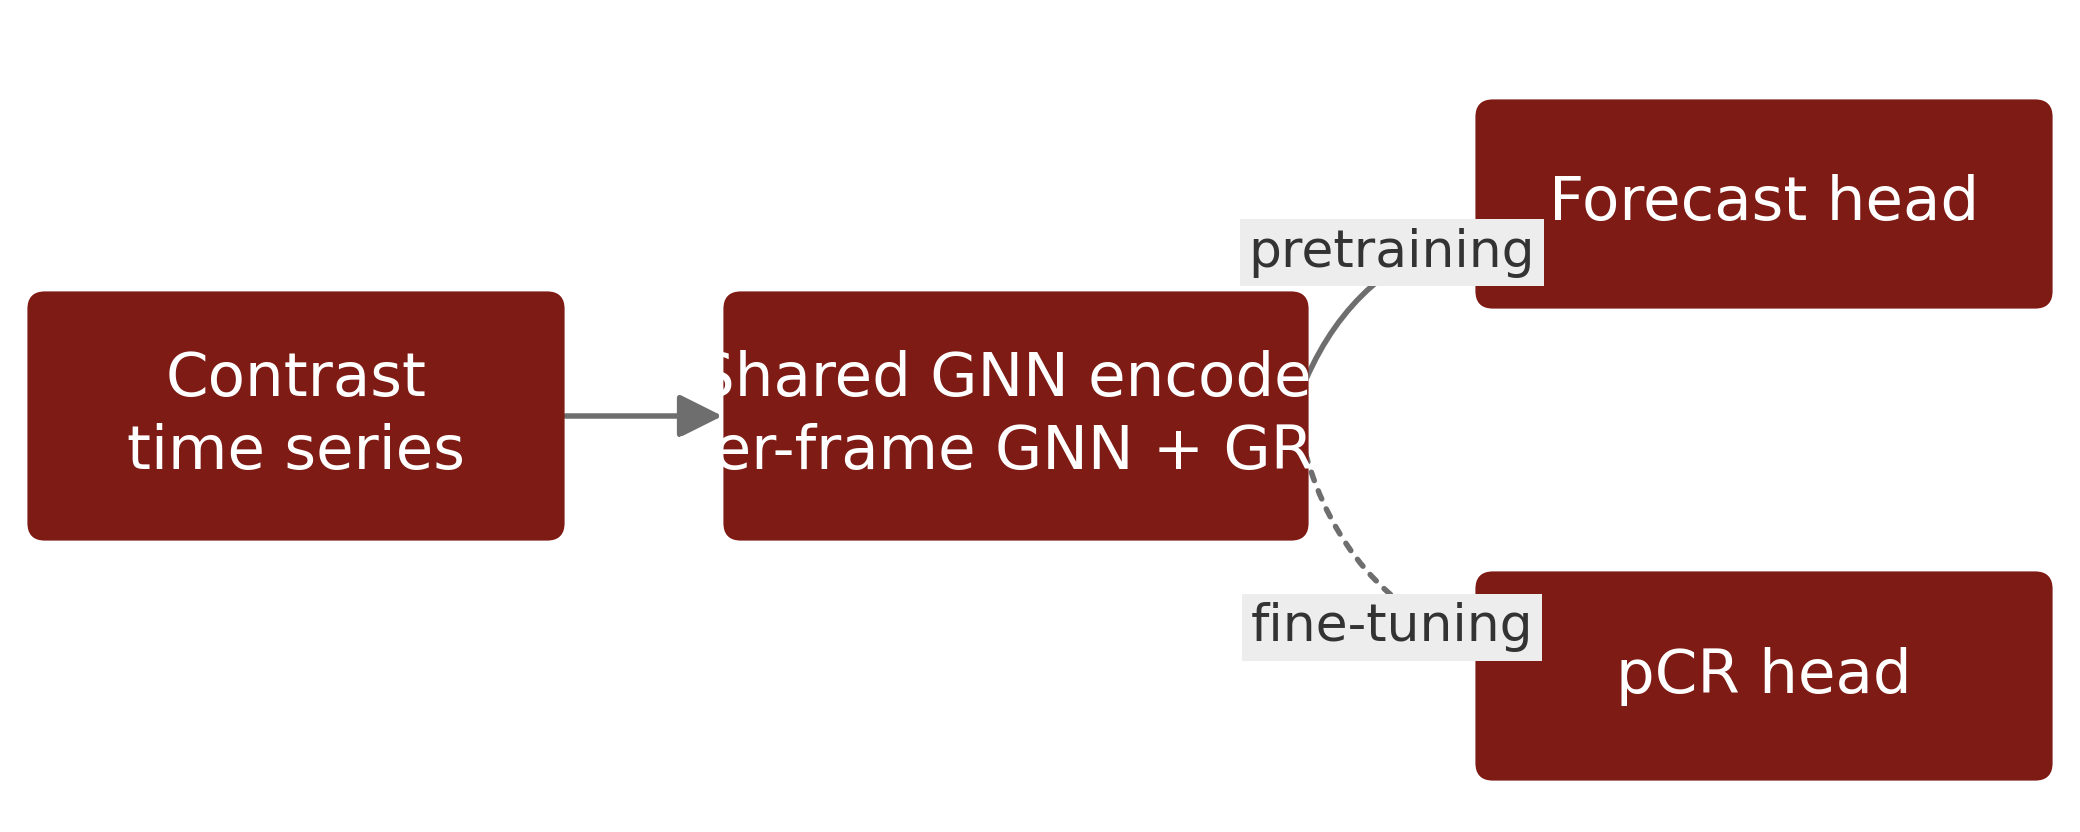
\includegraphics[width=0.62\linewidth]{contrast_pretrain_arch.png}\end{center}

  \vspace{2mm}
  Needing no labels is the point: pretraining can use $\approx$1{,}000 unlabelled
  ultrafast graphs, against 179 labelled ones.
  % docs/design/contrast_pretraining.md, sections 2 and 8a
  Built and validated end to end across all three graph representations.

  \vspace{3mm}
  \textbf{Pre-registered gates.} Beat trivial forecasters, then a graph-free
  forecaster, then random init on pCR by ${>}2\times$ the seed spread.

  \vspace{4mm}
  \tbdblock{26mm}{Gate results on ultrafast data.}{
    Forecasting MAE against the trivial and graph-free baselines, and
    pretrained-vs-random pCR AUC over ${\ge}5$ seeds.}
}

\block{\badgeontitle{1}\ \ Signal in the vessels?\ \ \color{LightYellow}YES}{
  UChicago ultrafast DCE-MRI, $N=179$, \textbf{vessels only} --- no tumour mask,
  no clinical variables. Pooled out-of-fold AUC, case-resampling bootstrap CIs.
  % experiments/uchicago_all_models/all_models_auc_ci.csv

  \vspace{2mm}
  \begin{tikzfigure}[Every vessel model clears chance; the control does not.]
    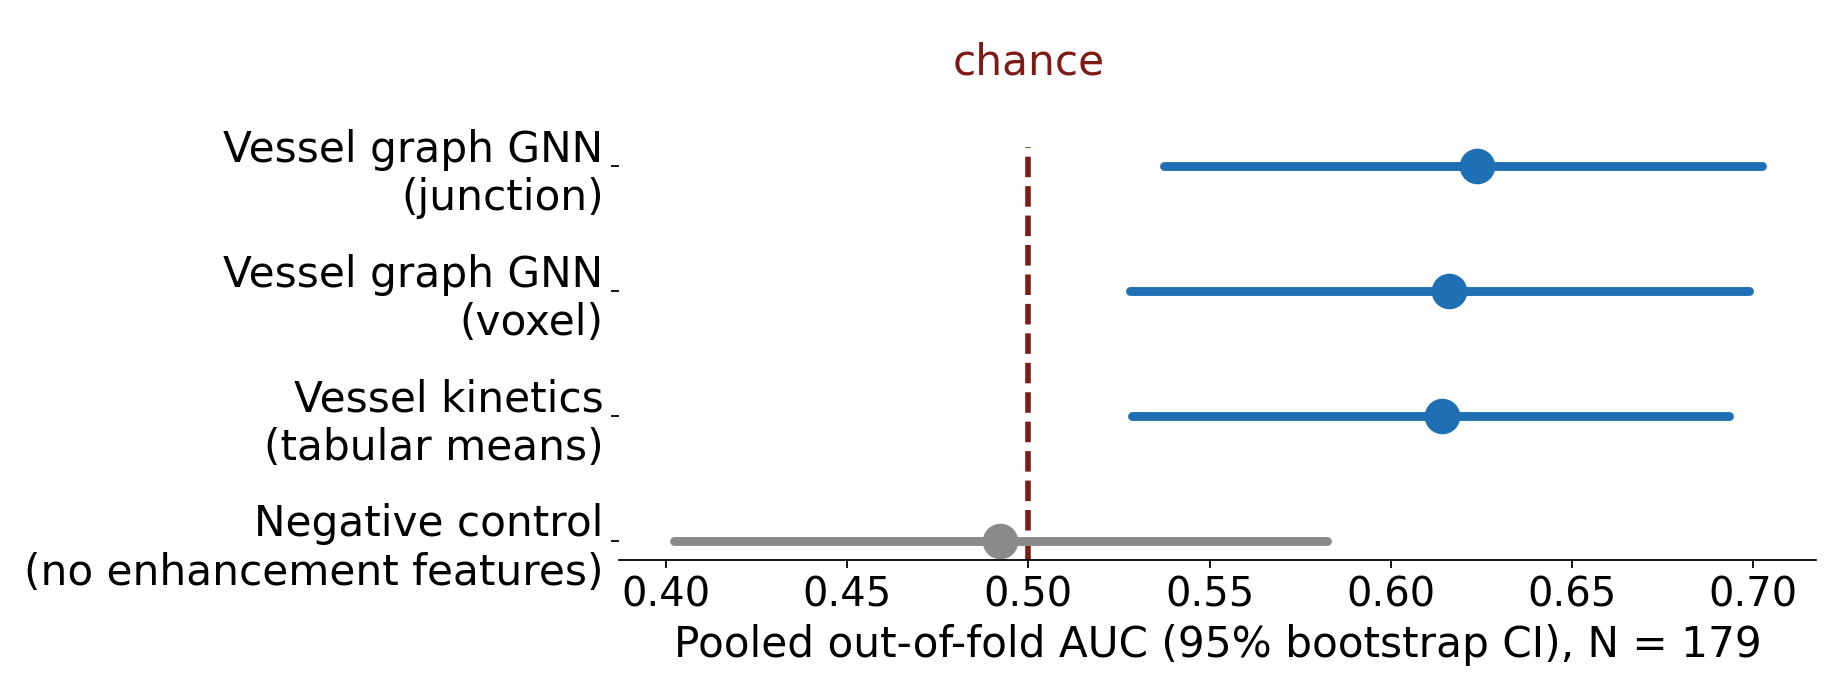
\includegraphics[width=0.64\linewidth]{q1_signal.png}
  \end{tikzfigure}

  \vspace{2mm}
  Bootstrap lower bounds clear 0.5 (0.526--0.538). A control model built from the
  only two node features that carry \emph{no} enhancement information --- peak
  time and radius --- sits at chance, so the signal is specifically in the
  contrast kinetics.
  % experiments/uchicago_graph_mode_floored/README.md ; all_models_auc_ci.csv

  Independently, on I-SPY2 \cite{garrucho_mamamia} ($n=808$), adding vessel
  features to clinical variables and tumour size raises AUC from
  $0.571 \pm 0.046$ to $0.606 \pm 0.028$ (XGBoost); the paired gain for logistic
  regression is $+0.024$, $p=0.025$.
  % results/issue118_baseline_arms_summary.csv ; results/README.md

  The signal only appeared after fixing a divide-by-near-zero baseline in the
  enhancement features: pooled AUC $0.49 \rightarrow 0.61$.
  % LAB_NOTEBOOK.md 2026-07-27 (correction) and 2026-07-28
}

\column{0.30}
\block{\badgeontitle{2}\ \ Does the graph add?\ \ \color{LightYellow}NOT YET}{
  \begin{tikzfigure}[Every paired interval contains zero.]
    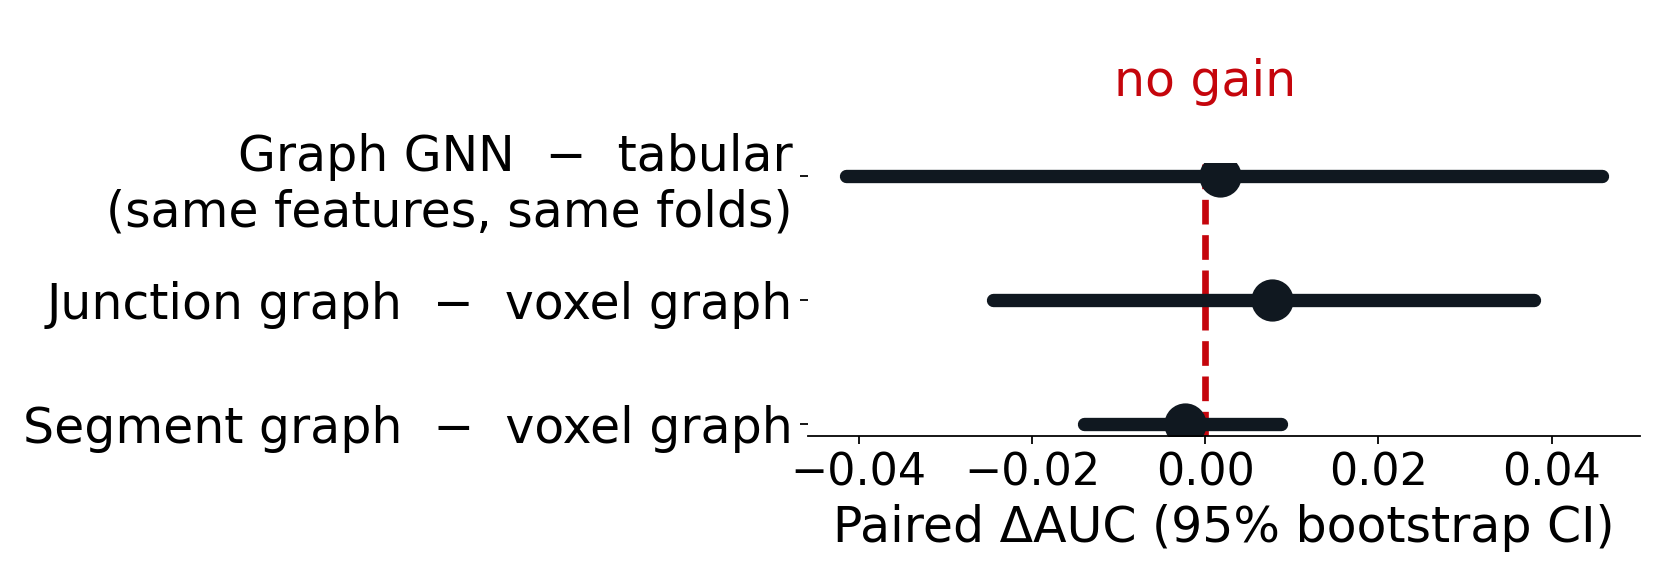
\includegraphics[width=0.86\linewidth]{q2_graph_delta.png}
  \end{tikzfigure}

  \vspace{2mm}
  Same features, same folds, paired bootstrap. The graph GNN does not beat a
  logistic regression on seven per-case feature means ($\Delta$AUC $+0.002$, 95\%
  CI $[-0.041, +0.046]$), and no structural representation beats the voxel graph.
  % experiments/uchicago_tabular_bar_floored/gate_paired_delta.csv
  % experiments/uchicago_graph_mode_floored/graph_mode_paired_delta.csv
  At $N=179$ that interval is $\pm0.04$ wide --- a smaller real advantage could
  not be detected here.

  \vspace{4mm}
  \tbdblock{26mm}{Sub-question 2 with temporal node representations.}{
    Paired $\Delta$AUC of a graph model that reads each node's full enhancement
    curve, against the same tabular bar on the same folds.}
}

\block{Conclusions}{
  \begin{itemize}[leftmargin=*, itemsep=1mm, topsep=0mm]
    \item Vessel kinetics predict pCR \textbf{from vessels alone}.
    \item The signal is in the \textbf{features}, not the representation.
    \item Graph topology, as encoded today, is not earning its cost.
  \end{itemize}

  \vspace{3mm}
  \textbf{Next.} Nodes get the curve, not six scalars; run the pretraining gates;
  add tumour features; grow the labelled cohort.
}

\block{References and acknowledgments}{
  \vspace{-1em}
  \begin{footnotesize}
  \printbibliography[heading=none]
  \end{footnotesize}

  \vspace{2mm}
  With thanks to \textbf{Dr.\ Anna Woodard} and the \textbf{UChicago Data
  Science Institute Summer Lab}.
}
\end{columns}

\end{document}
